\begin{figure*}[t]\centering
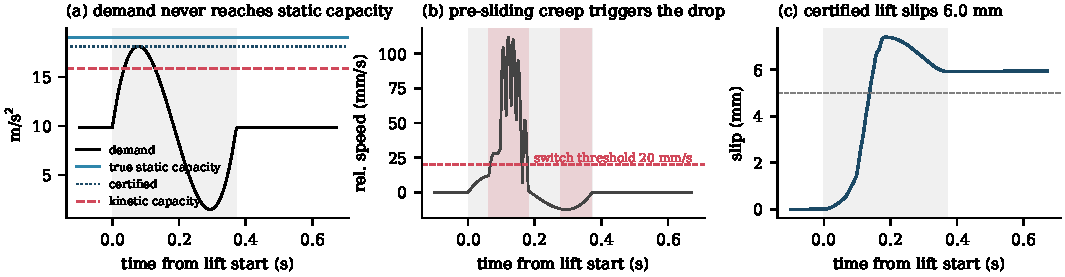
\includegraphics[width=\textwidth]{fig_e7case.pdf}
\caption{\textbf{When the certificate fails} (row E7, lift height 20\,cm, B5, $r=1.2$). (a) The demand peaks at 95\% of the
true static capacity, just below the certified level, so Coulomb friction should hold the rod. (b) The soft contact creeps
at up to 12\,mm/s before peak acceleration; the emulator's kinetic switch, which reads the relative speed with a one-step
lag that adds about 8\,mm/s here, fires at a true relative speed of 12\,mm/s (kinetic friction shaded), and the rod slides. (c) The certified lift ends 6\,mm low.}\label{fig:e7case}
\end{figure*}
